
We start with different variations of the \probstatic{}: we compare the two objectives
$\objcenter$ and $\objmedian$, and study the effects of relaxing various constraints in the problem.
Then, we consider the more realistic incremental version of the problem.

\subsection*{Individual vs social cost}
The $\objcenter$ objective models the individual cost, whereas the $\objmedian$ objective
is a better model of the social cost. 
Figure \ref{fig:kmed_vs_ksup} shows a comparison between these two objectives in Dataset A, as a function of
$k$, the number of facilities.
As one might expect, there is a significant tradeoff between these two objectives---the $\objcenter$ value
is almost three times the $\objmedian$ value for most values of $k$ for Sierra Leone; it is even higher for Liberia.
If there are difficult-to-reach areas (with high travel cost from other areas),
the $\objcenter$ can have a large value; the $\objmedian$ value might still be small if there are only
few such areas.  Therefore, these objectives need to be considered carefully during the planning process.

Next, we study if ignoring the connection costs for a small fraction of people can lead to a
significant improvement in the connection cost of the remaining population.
To explore this question, we develop two modified formulations of the \probstatic{} problem with the
$\objmedian$ objective.
First, how well does the $\objmedian$ solution do at minimizing the travel time of some fraction of 
the population of the population? 
Secondly, how well does the $\objmedian$ solution
do at maximizing the amount of people which obtain a specific travel time? 




\begin{figure}[h]
\centering
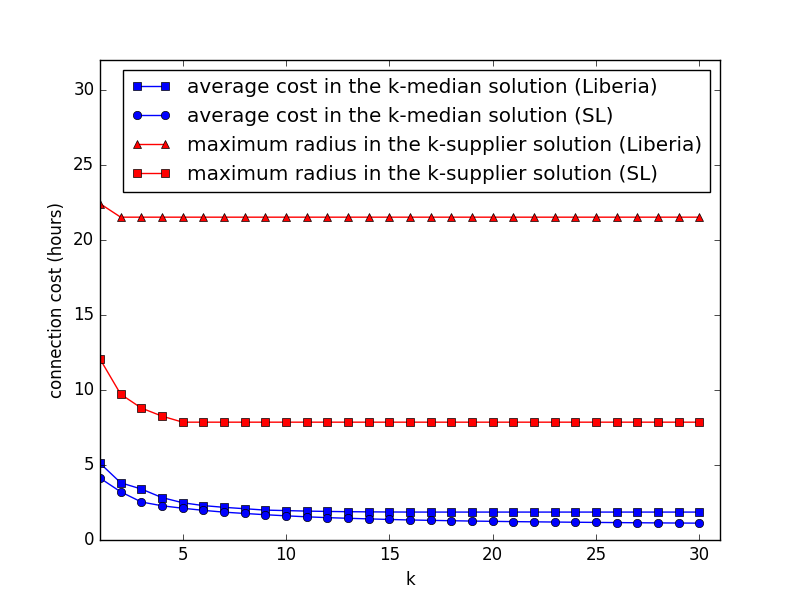
\includegraphics[width=0.5\textwidth]{new_figs/plot_A_kmed_vs_ksup.png}
\caption{Comparisons between the $k$-median and $k$-supplier objective functions for Dataset A.}\label{fig:kmed_vs_ksup}
\end{figure}


\subsubsection*{Minimizing cost of closest clients}
Recall that the goal here is:
given a cutoff distance $D$ and fraction $\epsilon$, minimize the average cost of the 
closest $(1-\epsilon)n$ clients subject to the constraint that those clients are all 
within distance $D$ of an open facility. 
In order to understand the impact of $D$ and $\epsilon$ in such a formulation, we compare the
fractional solution for this problem (by solving an LP), with the $\objmedian$ solution.
Figure \ref{fig:kmed_vs_LP1} shows the results for $D=6$ hrs and varying 
values of $\epsilon$, along with the solution to the $\objmedian$ objective (without any bound on $D$). 
For each value of $\epsilon$, we compared the cost of the top $(1-\epsilon)n$ clients 
(referred to as ``good'' clients) in the LP solution, against the cost of the top $(1-\epsilon)n$ 
clients in the ordinary $k$-median solution.
\red{clarify the previous sentence}
We observe that solutions allowing for violations only marginally 
improve the travel time of the top $(1-\epsilon)n$ clients over that of the $\objmedian$ solution.
These results indicate that, in practice, the ordinary $k$-median solution is already quite good with respect to 
these constraints, when $k$ is not too small.


\begin{figure}[h]
  \centering % left bottom right top
	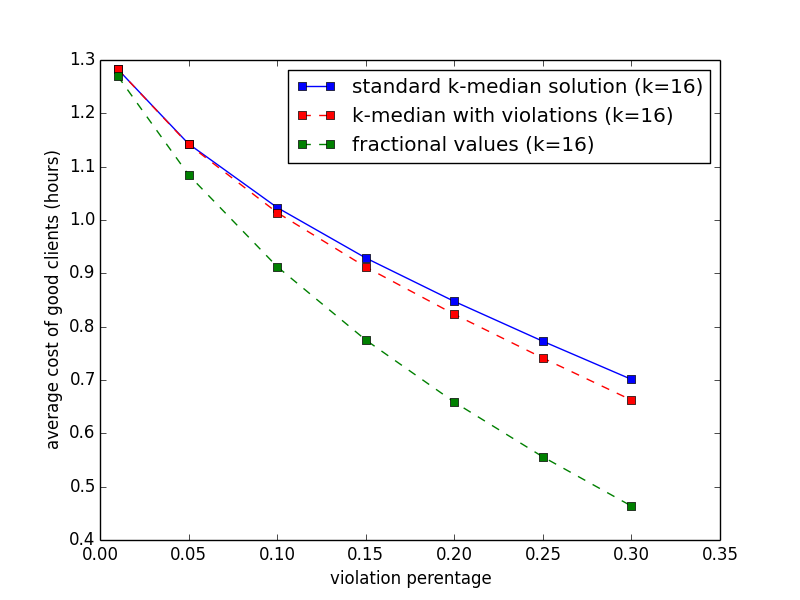
\includegraphics[width=0.48\textwidth]{figs/plotA16_violation.png}
	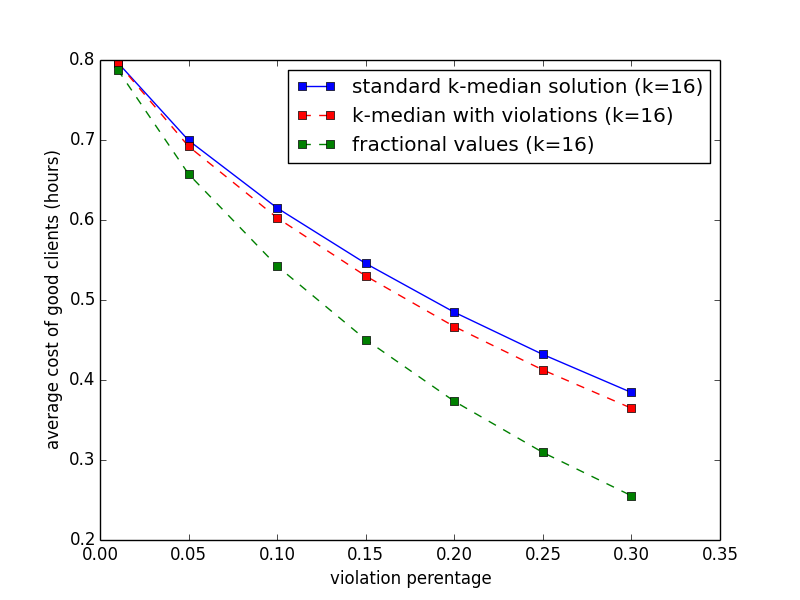
\includegraphics[width=0.48\textwidth]{figs/plotB16_violation.png}
\caption{Average cost of top $(1-\epsilon)n$ clients, for $k$-median solution and LP1 solution (fractional and best integral solution found) on Dataset A (left) and B (right). (Liberia)} 
	\label{fig:kmed_vs_LP1}
\end{figure}


\subsubsection*{Maximizing number of close clients}
Recall that here the goal is to maximize the number of clients which have a hospital within a given bound $D$.
Again, we study how the solution to the $\objmedian$ objective compares with a solution to such a formulation.
We solve an LP for this formulation, 
for $D$ varying from 2 to 7 hours, using $k=16$. We then take the solution to ordinary $k$-medain for $k=16$, 
and measure how many clients lie within distance $D$ for each value. 
Figure \ref{fig:LP2_AB} shows that the $k$-median solution comes quite close to the fractional solution.
These results again suggest that the $k$-median solution is already quite robust, in that it already does 
a good job maximizing the number of clients within distance $D$, for many values of $D$ simultaneously. 
Our conclusion in this subsection is that it is only marginally beneficial to exclude any of the population as outliers. The ordinary $k$-median problem already yields a good quality solution. 

\begin{figure}[h]
  \centering % left bottom right top
    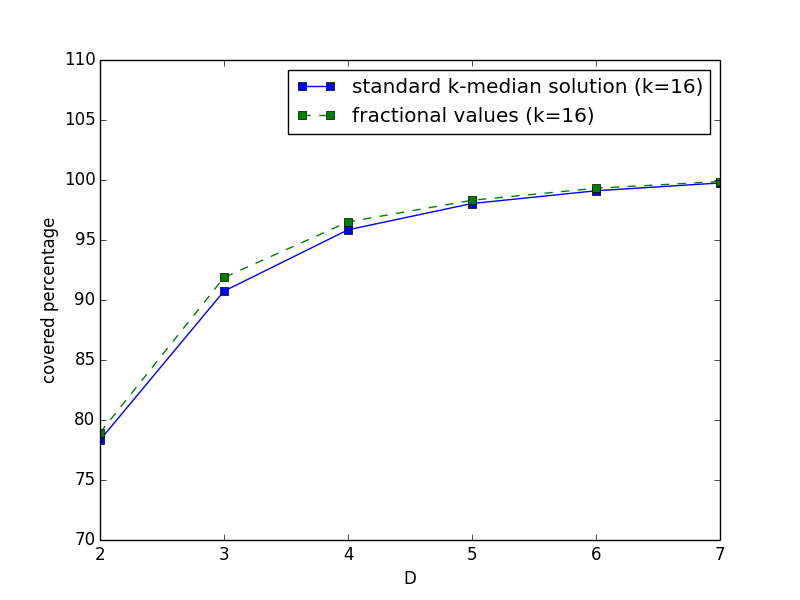
\includegraphics[width=0.4\textwidth]{figs/plotA16_min_violation.png}
	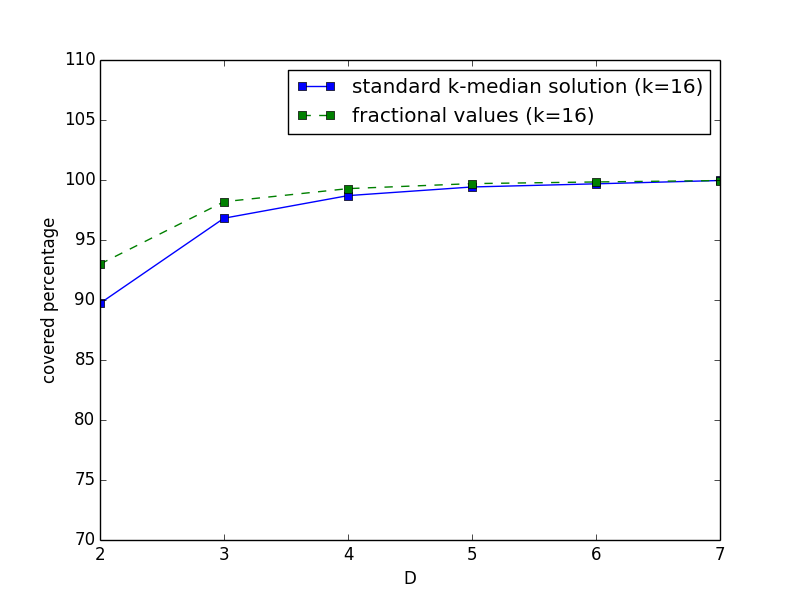
\includegraphics[width=0.4\textwidth]{figs/plotB16_min_violation.png}
\caption{Our results of solving LP2 for Dataset A (left), and B (right). (Liberia)} 
	\label{fig:LP2_AB}
\end{figure}



\subsection*{Kernel facilities}
We run algorithm \algokernelkmed{} on datasets A and B \red{(averaged across all subinstances, $r = 30$)}.
Figure \ref{fig:coreset_A_and_B} shows the frequencies of facilities, sorted in decreasing order.
The figure shows that there are many facilities which occur in most of the solutions, and many facilities which are rarely used in any solution.
Recall that we define the $\ell$-kernel as the $\ell$ facilities which have the highest frequencies. For example, the $10$-kernel for Dataset A is strong, as all its facilities occur in at least $90$\% of the solutions. Dataset B has weaker kernels, possibly because it is an average over multiple possible demand sets. Comparing the kernels of Datasets A and B, there is no apparent correlation. Our explanation is that the most useful facilities for the population data are spread out across the country.


\begin{figure}[h]
  \centering % left bottom right top
    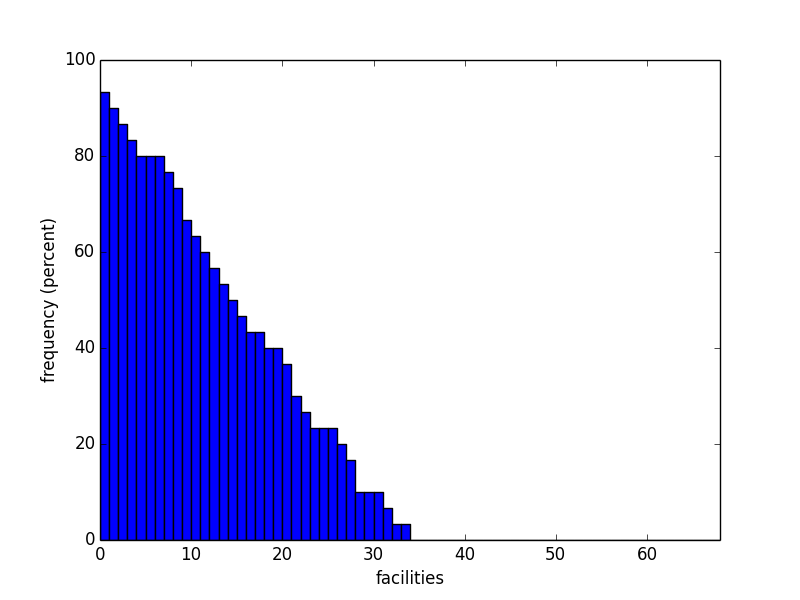
\includegraphics[width=0.4\textwidth]{figs/coresetA.png}
        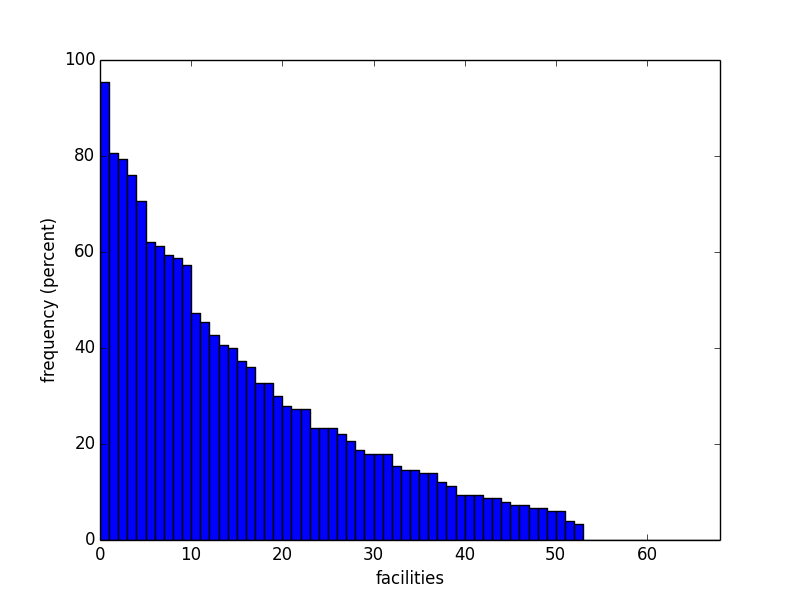
\includegraphics[width=0.4\textwidth]{figs/coresetB.png}
\caption{Facility frequencies for Dataset A (left) and Dataset B (right), sorted by frequency. (Sierra Leone)}
        \label{fig:coreset_A_and_B}
\end{figure}



\begin{figure}[h]
  \centering
    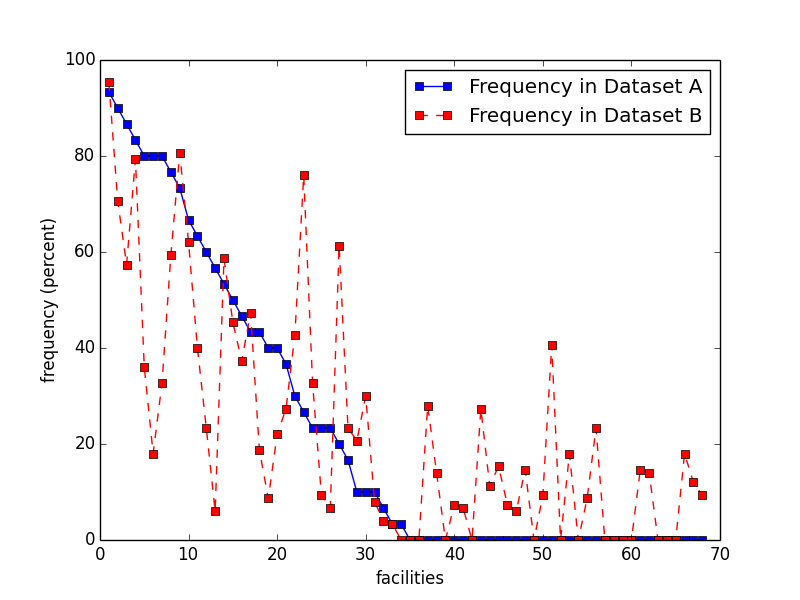
\includegraphics[width=0.4\textwidth]{figs/coreset_AB.png}
    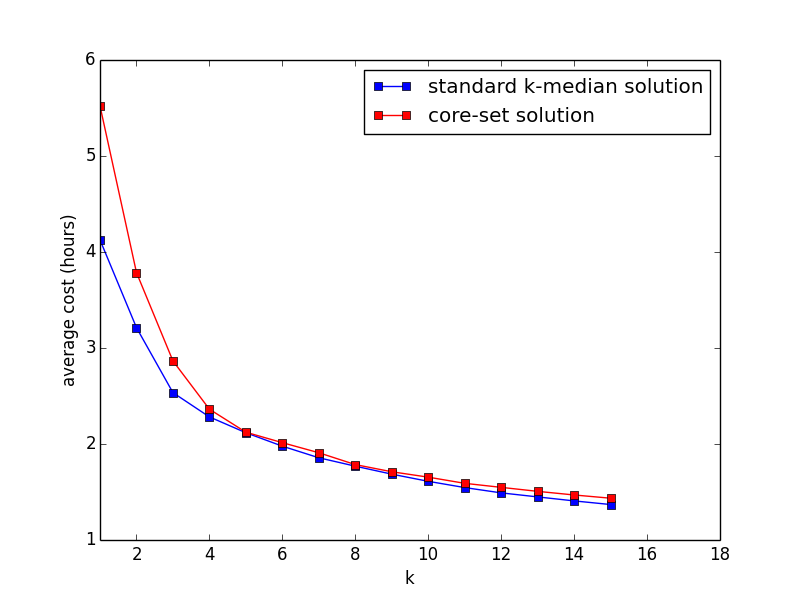
\includegraphics[width=0.4\textwidth]{figs/core_only.png}
\caption{
(a) Facility frequencies compared between Dataset A and B.
(b) Performance of the optimal $k$-median solution vs. the kernel solution of size $k$, in dataset A. (Sierra Leone)
} 
        \label{fig:coreset_AB}
\end{figure}





\subsection*{Importance of forecasting}
The epidemic dynamics drives the demand for healthcare resources, and it seems
likely that planning using forecast demands would give improvements over not
considering such information at all. At the same time, there is uncertainty
in forecasts using all current methodologies, especially at a high
spatio-temporal scale \cite{chakraborty:sdm14}.
In order to evaluate the effect of forecasting,
we consider solutions for instance $C$ computed in three different
ways: (1) the optimum solution, denoted by $OPT_C$;
(2) the solution computed by using $p^B_j$ as the demands;
and (3) the solution computed by using $p^A_j$ as the demands.
Figures \ref{fig:ABC_L} and \ref{fig:ABC_L} show this comparison for several values of $k$.

%In the $k$-median problem, we examine demands at a single time step and find an optimal solution. But as the outbreak evolves, the demands shift and the solution will no longer be optimal. In the following experiment, we suppose that the solution is generated based off of t=0, 1, or 2 data, and then measure how well that solution performs given the t=2 demand. For t=0, this means determining the facility set pre-outbreak, based on population alone. For t=1, this means either waiting until the t=1 time point to determine the facility set, or using accurate modeling to predict the t=1 situation. For t=2, this again means either waiting until t=2 to actually determine the facility set, or using accurate modeling. All 3 of these solutions are then applied to the t=2 demand set and the average distance measured. Using the t=2 data will by definition give the best-possible solution, so the interest is in comparing the t=2 solution against the t=0 and 1 solutions. Figure \ref{fig:ABC} shows this comparison for several values of $k$.


\begin{figure}
    \centering
       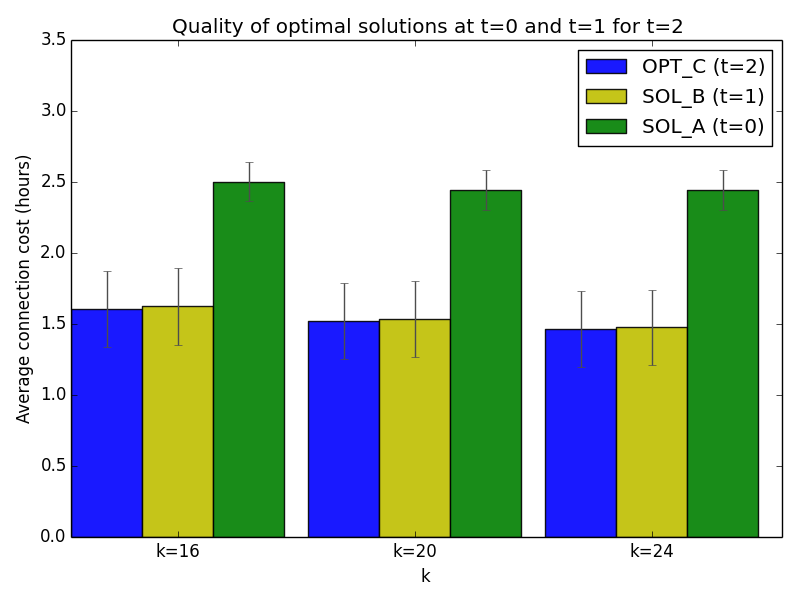
\includegraphics[width=0.40\textwidth]{new_figs/plotABC_L.png}
       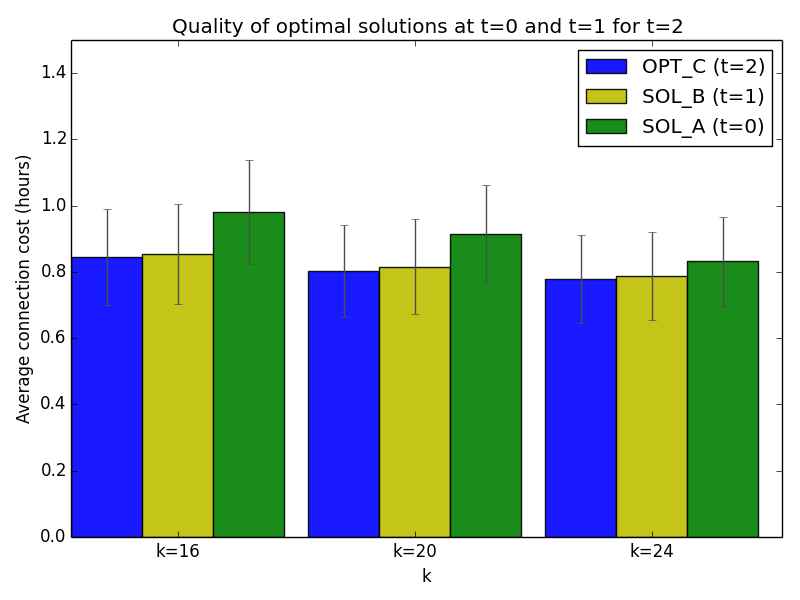
\includegraphics[width=0.40\textwidth]{new_figs/plotABC_SL.png}
    \caption{Quality of the solutions at time $t=0$ and $t=1$ at time $t=2$ for Liberia (left) and Sierra Leone (right). }
\label{fig:ABC_2countries}
\end{figure}

\begin{figure}
    \centering
       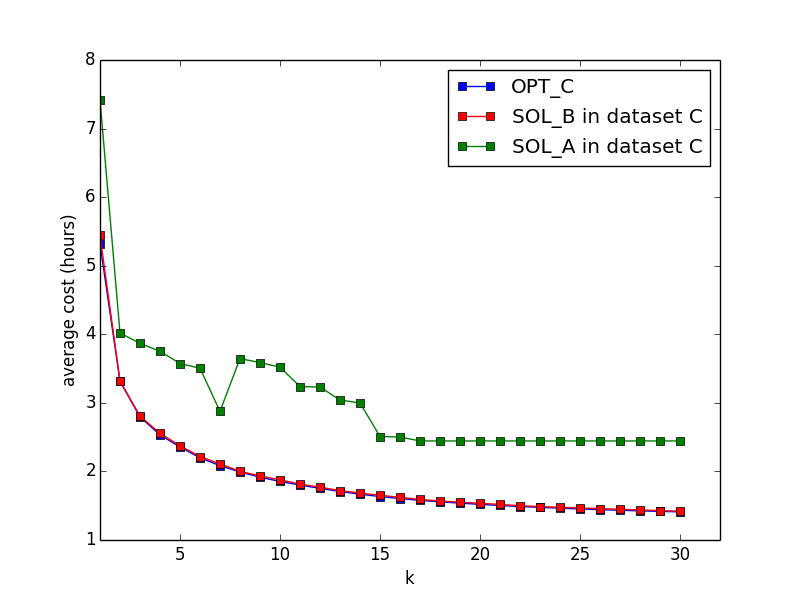
\includegraphics[width=0.40\textwidth]{new_figs/ABC_average_L.png}
       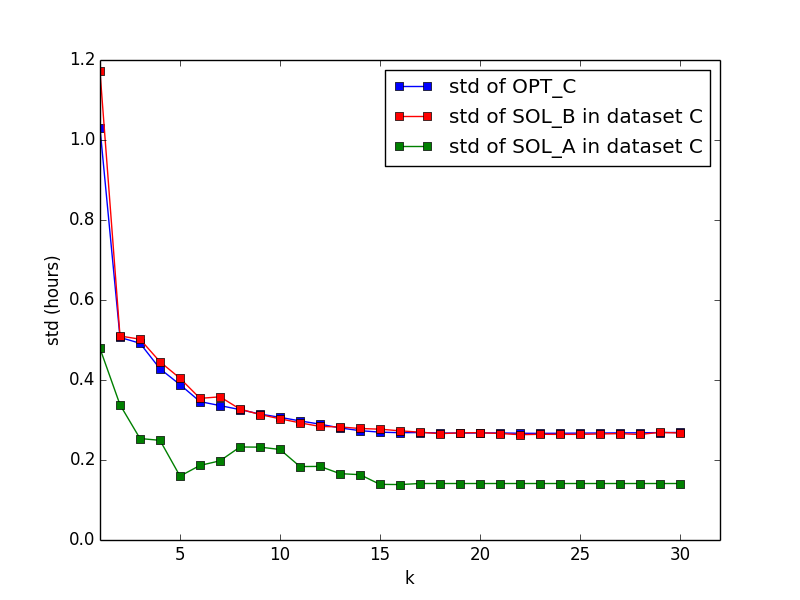
\includegraphics[width=0.40\textwidth]{new_figs/ABC_std_L.png}
    \caption{Compare solutions calculated at each time. (Liberia)}
\label{fig:ABC_L}
\end{figure}

\begin{figure}
    \centering
       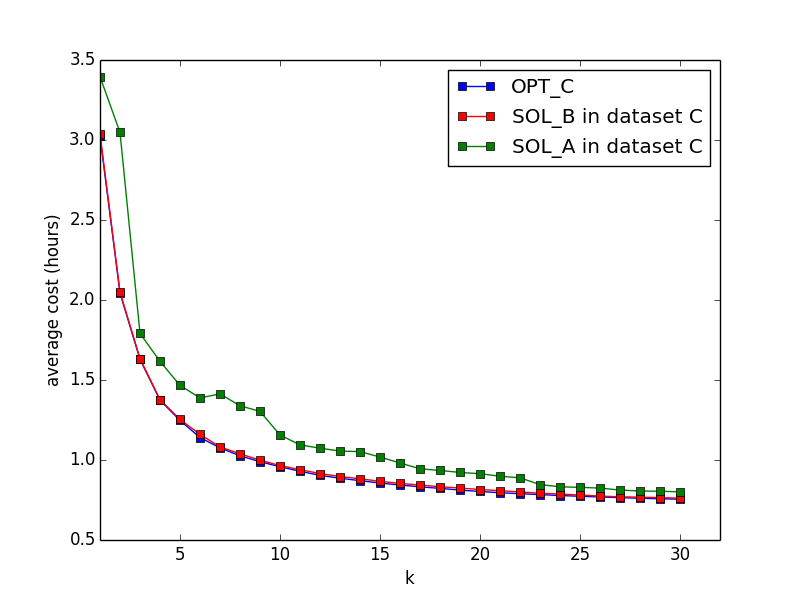
\includegraphics[width=0.40\textwidth]{new_figs/ABC_average_SL.png}
       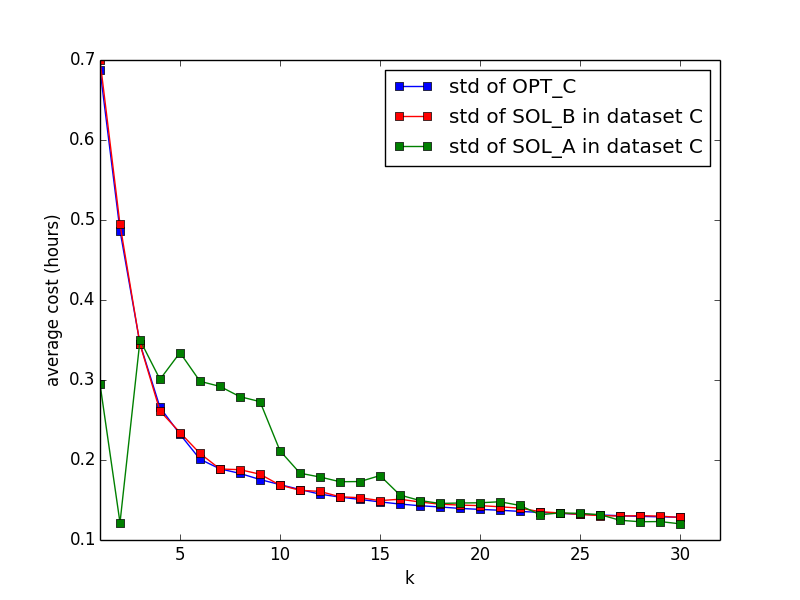
\includegraphics[width=0.40\textwidth]{new_figs/ABC_std_SL.png}
    \caption{Compare solutions calculated at each time. (Sierra Leone)}
\label{fig:ABC}
\end{figure}

\noindent
Our main observations here are
\begin{itemize}
\item
We find that the solution $p^B_j$ computed using demands from B is significantly better than the
solution $p^A_j$ computed using the demands from instance A. For instance, as Figure \ref{fig:ABC_L}
shows an almost 40\% reduction in the average cost objective, for $k=16$ facilities.
Indirectly, this suggests that instead of using static population demands, if we were able to obtain 
forecasts, this would give much better solutions.
%Deciding the facility locations by taking forecasted incidence rates can significantly
%improve the quality of the solution, especially when the number of facilities is low.
%For instance, if 5 facilities are to be placed, using the forecasted demand can give
%close to 10-15\% reduction in the average travel time, compared to solutions that do
%not take forecasts into account.
%With the new dataset B (t=1), t=1 behaves very similarly to t=2. There is some difference between t=0 and t=2, which vanishes as $k$ increases. ``Does the small difference between T1 and T2 solutions imply that the disease had reached its maximum spatial distribution before exponential growth began?''
\item
The precise benefits from using forecasting are hard to guage without using results from specific
forecasting methods; however, that can bring in additional difficulties relating to the performance of the
forecasting methods themselves. Instead, we examine the effects of uncertainty on demands on the
performance, which give us some insights into how well the forecasting methods should be.
We discuss the effects of uncertainty below for $k=16$ facilities.
\begin{itemize}
        \item We perturb all distances by a random $\delta \in [-1.5, +1.5]$ (hours), 
and solve the $k$-median instances (repeat $20$ times). We find that 15 out of the 16 facilities appear
in the solutions for all the 20 trials.

        \item Repeat the experiment with $\delta \in [-1, +1]$. Result : $15/16$ facilities appear in all $20$ trials; there's one facility appearing in $\approx 80\%$ of the trials.

        \item Perturb each distance $w_{ij}$ by $w_{ij} \gets w_{ij} + \delta w_{ij}$ where $\delta \in [-0.35, +0.35]$. Result : $15/16$ facilities appear in all $20$ trials; there's one facility appearing in $\approx 10\%$ of the trials.
\end{itemize}
\end{itemize}



\subsection*{Performance of a hybrid approach}
We have seen in the last subsection that using a set of facilities completely based on the static population information would be bad as the epidemic spreads in the future. On the other hand, it is crucial to ``pre-open'' a few hospitals to control the disease at the early stage of the epidemic. Here we consider a hybrid approach which opens $\ell$ facilities at timestep $t=0$, and $k-\ell$ additional facilities at timestep $t=2$. This solution will be evaluated on Dataset C.

How should we choose the set of important facilities to pre-open at time $t = 0$? In our below results, this set will be chosen as the $\ell$-kernel in Dataset A (using \textsc{KernelkMed}) with $\ell = 5$ facilities. The results show that once $k$ is a little higher than the kernel size, the solutions obtained are quite good; they are very close to the optimal solutions based entirely on the later time point. Determining the entire solution based on Dataset A on the other hand leaves a significant gap in optimality at a later time point.


\begin{figure}[h]
    \centering
       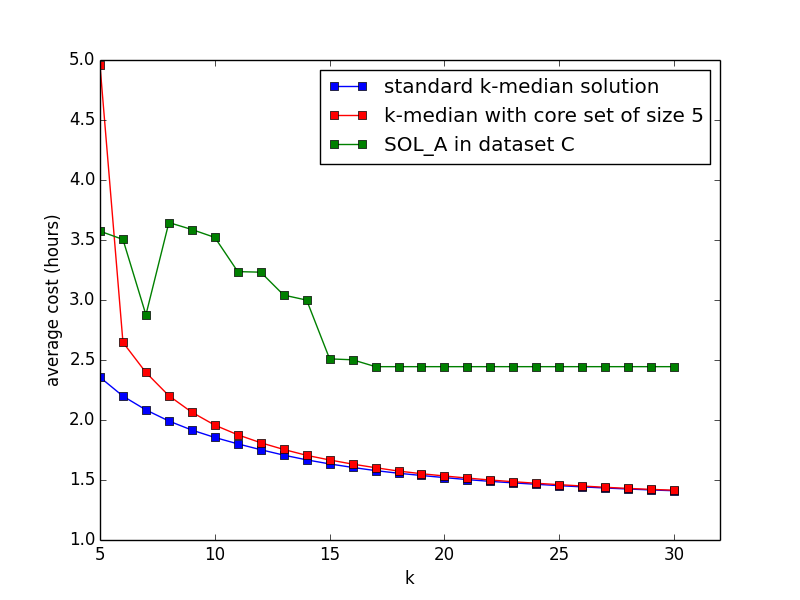
\includegraphics[width=0.40\textwidth]{new_figs/plotC_hybrid_freq_L.png}
       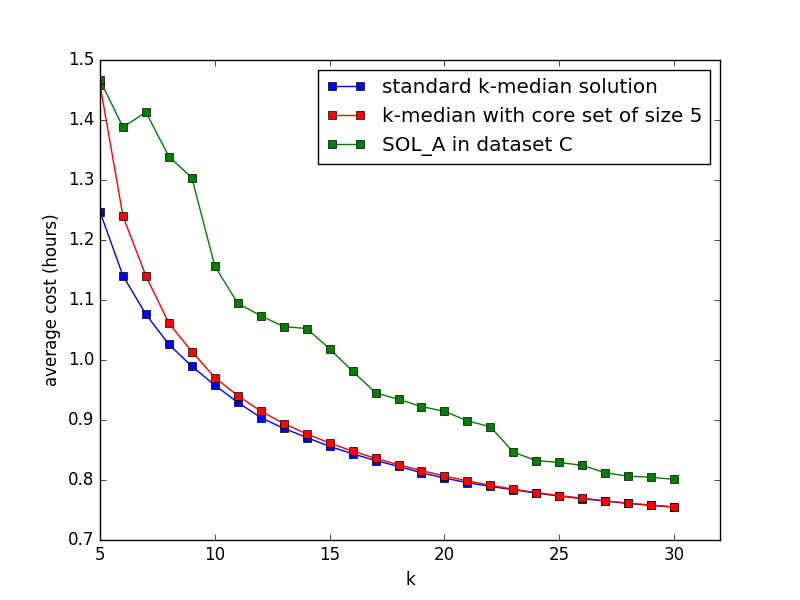
\includegraphics[width=0.40\textwidth]{new_figs/plotC_hybrid_freq_SL.png}
    \caption{Hybrid solutions for Liberia (left) and Sierra Leone (right).}
\label{fig:hybrid}
\end{figure}


\subsection*{Incremental facility location}
\red{this overlaps with the hybrid version above. Maybe merge both?}
In this section, we summarize our numerical results for the incremental hospital location problem. Recall that $t_1, t_2, \ldots$ are the times after $1$ week, $2$ weeks, etc from the start of the epidemic. We exploit the property of kernel facilities in the following manner: for the first $s-1$ time points (weeks), $t_1, \ldots, t_{s-1}$, we only use the kernel with uniform capacity $cap_1$. Starting from time $t_{s}$, we build $k'$ additional hospitals at time points  $t_s, t_{s+w}, t_{s+2w}, \ldots$ for some $w \in \mathbb{N}$. In other words, we are able to build $k'$ additional facilities after every $w$ weeks starting from time $t_s$. These new hospitals will have uniform capacity $cap_2$.


\begin{itemize}
\item
Figure \ref{fig:online1} compares the incremental solution with 
$s=1$, $w=2$, $k=5, k' = 2$, $cap_1 = cap_2 = 100$, with the static fractional solution
(which serves as a lower bound). We find that the solutions are really close, after about 5 weeks.
\item
The performance of the incremental approach depends on the initial capacity, $cap_1$, as shown
in Figure \ref{fig:online2}. If $cap_1$ is too low, this can cause spikes in the average cost
at some subsequent time, when the patient demand peaks.
\item
Another important determinant for the performance of the incremental algorithm is the
number $k'$ of facilities opened at each time. Figure \ref{fig:online3} compares two different
policies, namely (i) one every two weeks, starting at week 10, and
(ii) two each week, starting week 1. As one would expect the former has a much
higher cost, especially in the early stages of the epidemic.
\end{itemize}

\begin{figure}[h]
  \centering % left bottom right top
    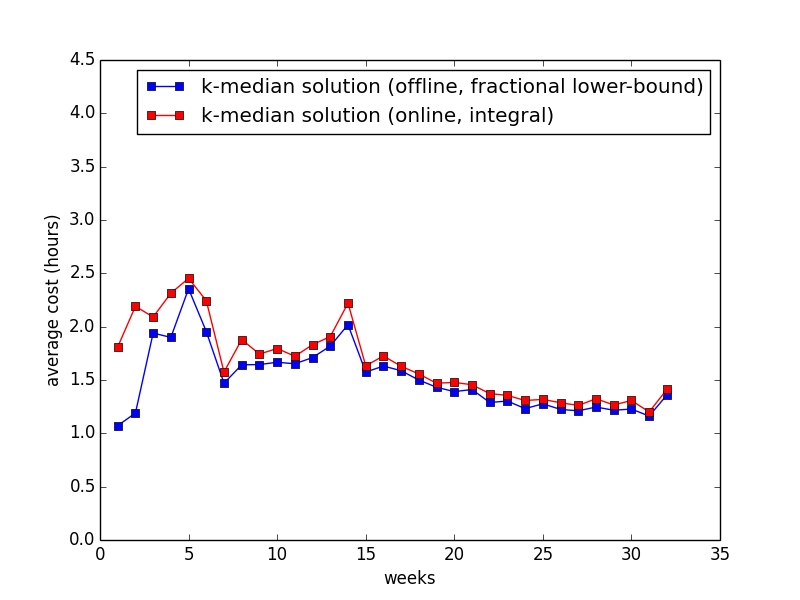
\includegraphics[width=0.30\textwidth]{figs/plot_kmed_CAP100.png}
    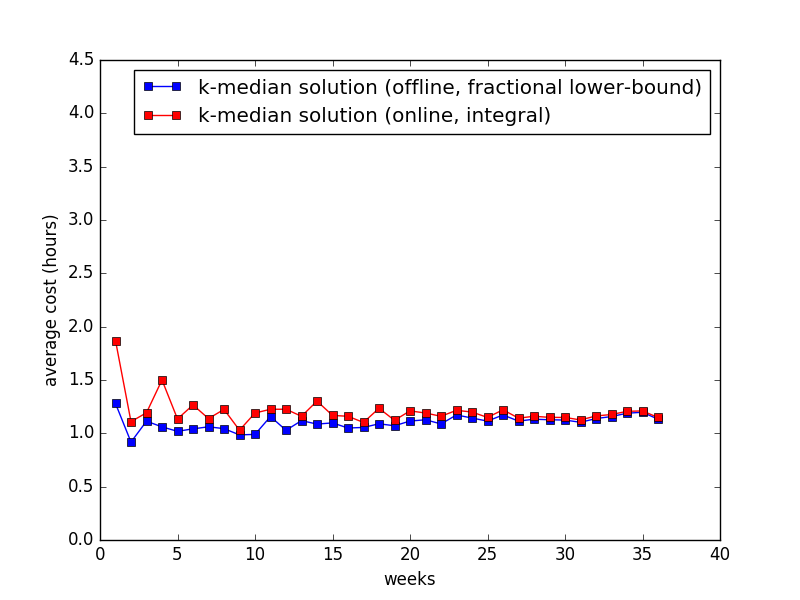
\includegraphics[width=0.30\textwidth]{figs/plot_kmed_CAP100_SL.png}
    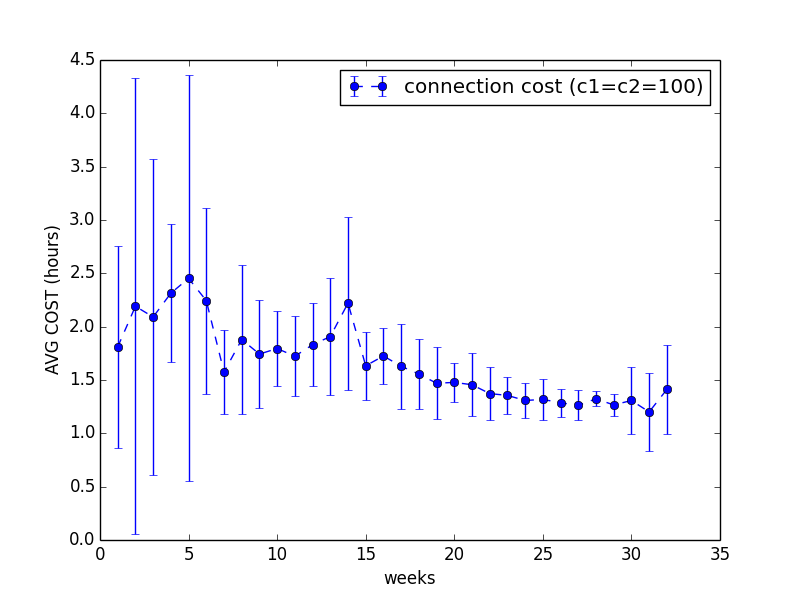
\includegraphics[width=0.3\textwidth]{figs/plot_online_cap100.png}
    \caption{Comparing the static and incremental strategies for
$s=1$, $w=2$, $k=5, k' = 2$, $cap_1 = cap_2 = 100$ for
(a) Liberia, and (b) Sierra Leone.
The variance in the solution costs over multiple iterations is shown in (c).}
\label{fig:online1}
\end{figure}

\begin{figure}[h]
  \centering % left bottom right top
    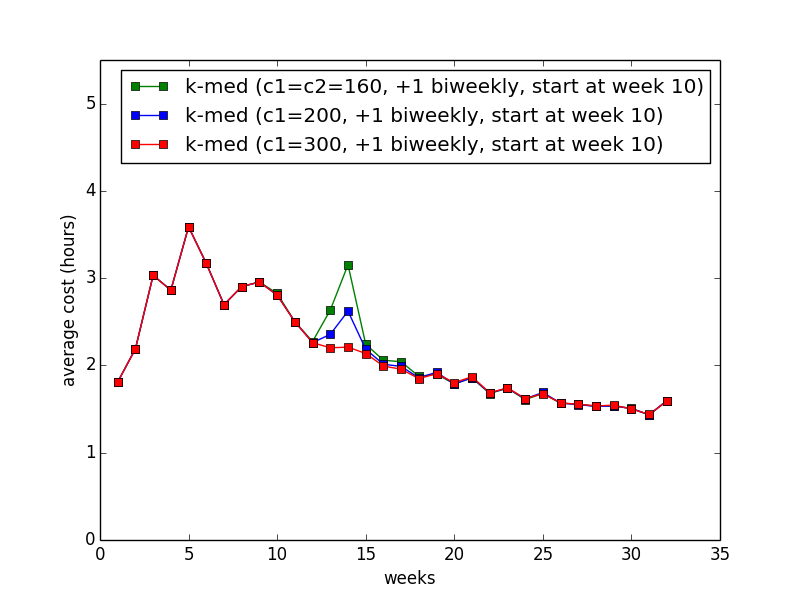
\includegraphics[width=0.45\textwidth]{figs/plot_kmed_c1.png}
    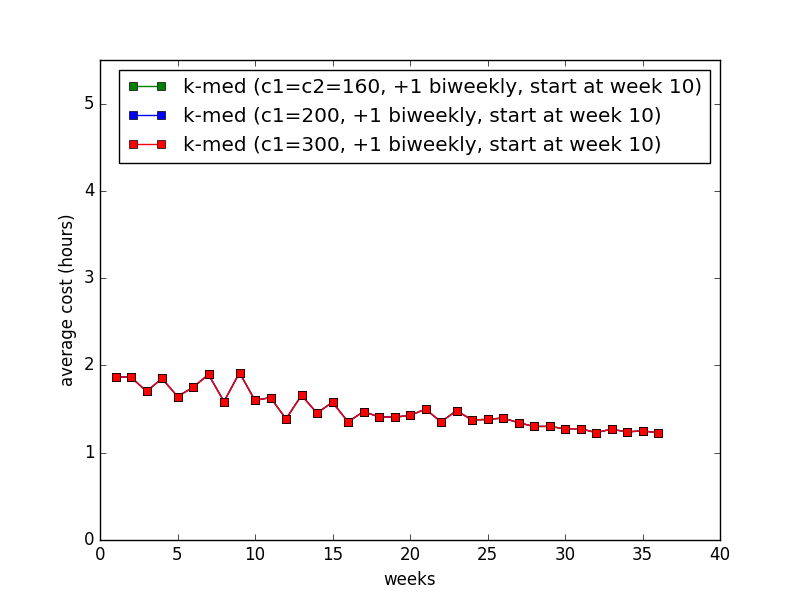
\includegraphics[width=0.45\textwidth]{figs/plot_kmed_c1c2_SL.png}
    \caption{Effect of the initial capacity $cap_1$ on the incremental solution, with
parameters $s = 10, w = 2, k' = 1, cap_2 = 160$, for (a) Liberia, and (b) Sierra Leone.}
\label{fig:online2}
\end{figure}

\begin{figure}[h]
  \centering % left bottom right top
    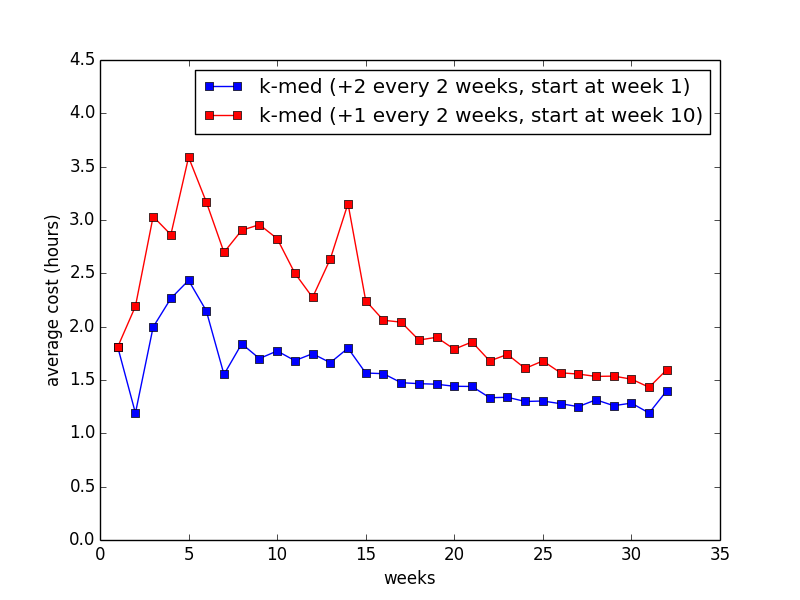
\includegraphics[width=0.45\textwidth]{figs/plot_kmed_CAP160_s1_s10.png}
    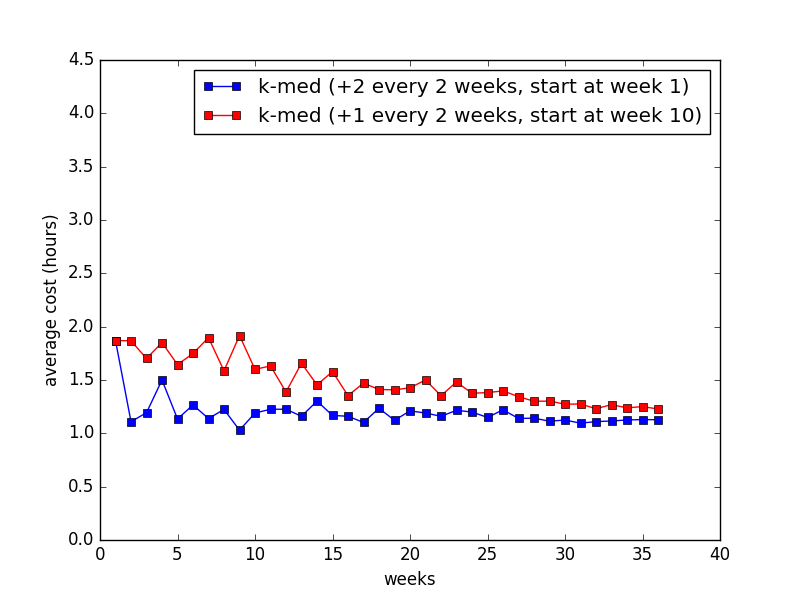
\includegraphics[width=0.45\textwidth]{figs/plot_kmed_CAP160_s1_s10_SL.png}
    \caption{Two different opening policies, with kernel size = $5$, for
(a) Liberia and (b) Sierra Leone.}
\label{fig:online3}
\end{figure}


